\documentclass{article}

\usepackage[utf8]{inputenc}
\usepackage{longtable}
\usepackage{authblk}
\usepackage{adjustbox}
\usepackage{natbib}

%Creación de títulos del artículo
\title{Índices de Desarrollo Humano de Colombia}

\author[1]{\normalsize Andrés Esteban Acero}
\affil[1]{\small  Doctorado en Ingeniería Industrial, Facultad de Ingeniería,Universidad de los Andes\\
\texttt{{ae.acero539@uniandes.edu.col}}}


\date{29 de Junio de 2018}



\usepackage{Sweave}
\begin{document}
\Sconcordance{concordance:Articulo1.tex:Articulo1.Rnw:%
1 20 1 1 0 11 1 1 16 8 1 1 5 1 2 5 1 1 10 1 2 5 1 1 20 1 2 6 1 1 6 12 0 %
1 2 1 1 1 9 13 0 1 2 2 1 2 2 9 1 1 5 1 1 1 4 31 0 1 2 8 1 1 10 1 1 1 12 %
2 1 1 16 1 3 8 1}


\maketitle

\begin{abstract}
El índice de desarrollo humano es uno de los indicadores compuestos de desarrollo socio-económico más utilizado en el mundo.Un estudio detallado de los índices de desarrollo humano en el mundo ha mostrado que esta medida, a pesar de sus detractores, refleja un enfoque integral para el estudio de las condiciones de un país.Además, se mantiene como un reflejo de los esfuerzos de recuperación democrática y humanitaria.  Sin embargo, estudios detallados regionales acerca del uso de este indicador, en especial en países en desarrollo, son pocos y con niveles de análisis inadecuados. Por tanto, este artículo hace un análisis detallado del índice de desarrollo humano para cada uno de los departamentos (estados) de Colombia. Este análisis incluye predicciones acerca de las características demográficas que explican este índice, así como agrupamiento de los niveles de desarrollo regional de acuerdo con este índice. De este estudio se concluye que existen tres niveles diferentes de desarrollo, en los cuales un efecto de centro-periferia es evidente, con zonas de desarrollo menor entre estas dos.
\end{abstract}

\section*{Introducción}
El índice de desarrollo humano, de acuerdo con \cite{sales_proposal_2018}

Comencemos viendo que hay en la sección \ref{univariada} en la página \pageref{univariada}.
\clearpage

\section{Exploración Univariada}\label{univariada}
En esta sección exploro cada índice.


\begin{figure}[h]
\centering
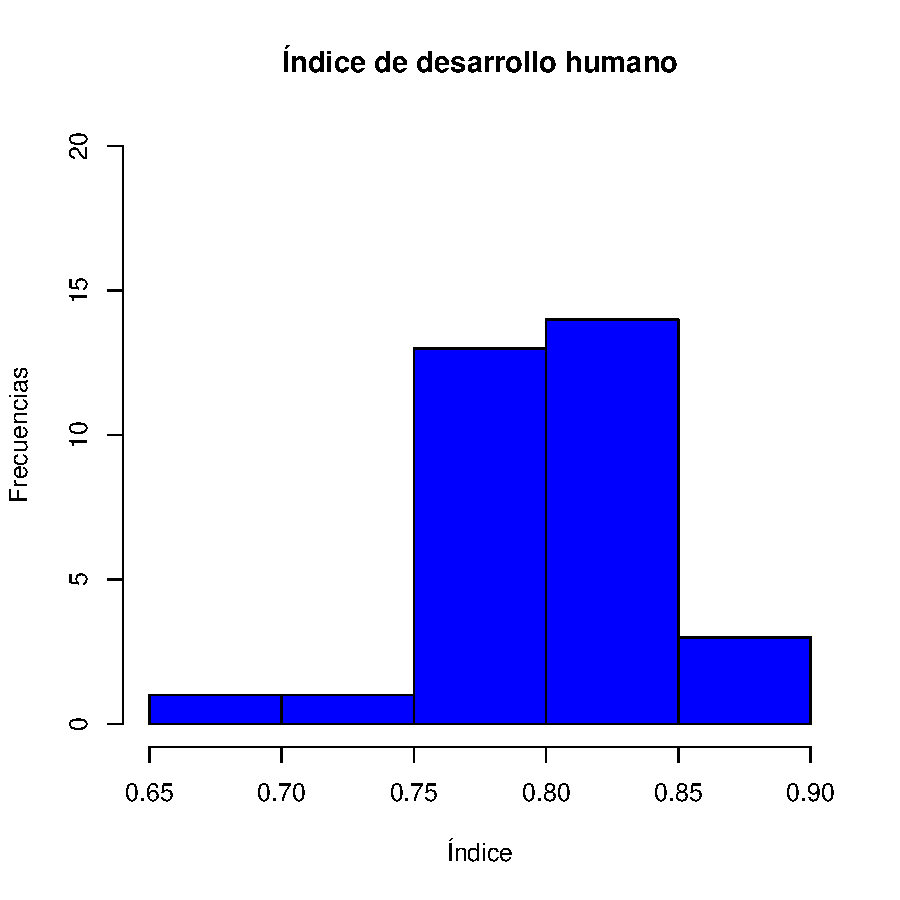
\includegraphics{Articulo1-histIDH}
\caption{Índice de desarrollo humano}
\label{barplots}
\end{figure}

\begin{figure}[h]
\centering
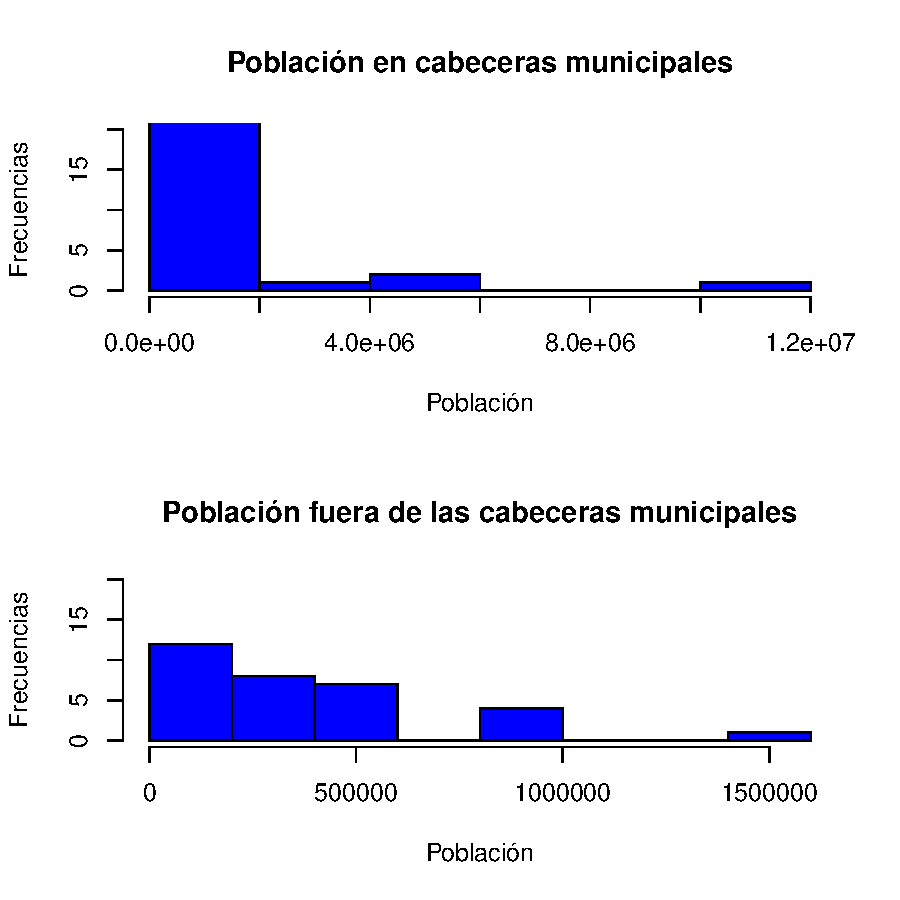
\includegraphics{Articulo1-histPOB}
\caption{Estadísticas demográficas}
\label{barplot2}
\end{figure}

\begin{figure}[h]
\centering
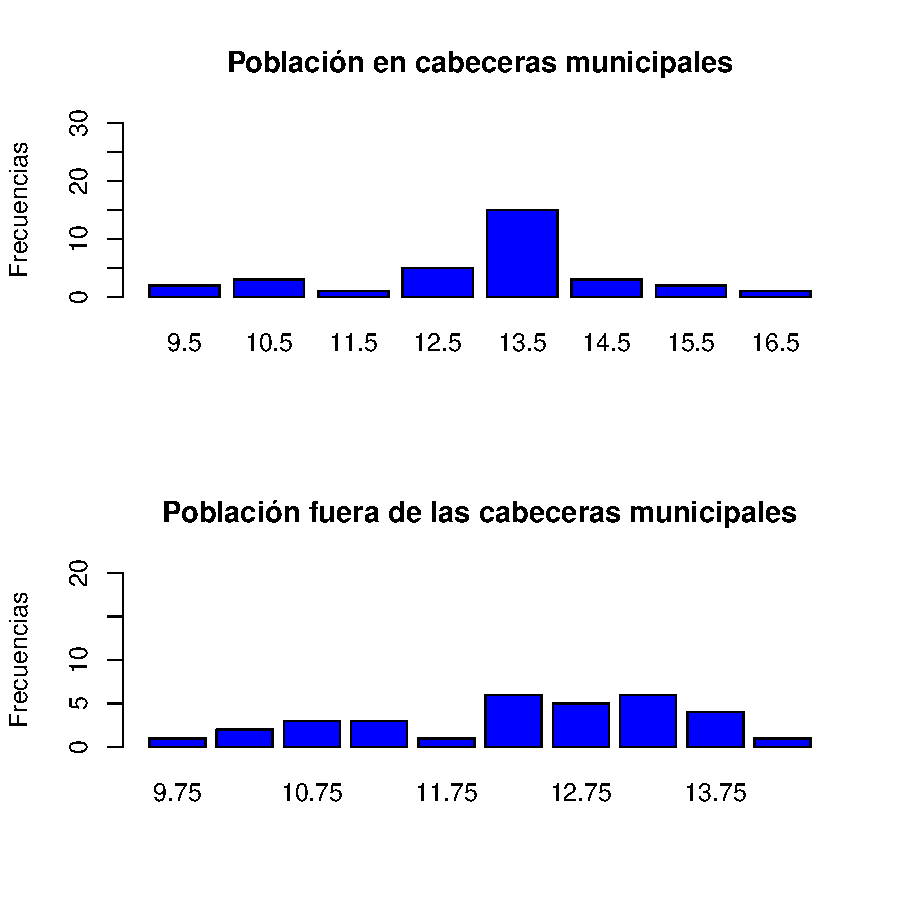
\includegraphics{Articulo1-histNOR}
\caption{Estadísticas demográficas Normalizadas}
\label{barplot3}
\end{figure}
\clearpage
\section{Exploración Bivariada}
En este trabajo estamos interesados en el impacto de los otros indices en el nivel de Democracia. Veamos las relaciones bivariadas que tiene esta variable con todas las demás:

% Table created by stargazer v.5.2.2 by Marek Hlavac, Harvard University. E-mail: hlavac at fas.harvard.edu
% Date and time: vie, jun 29, 2018 - 07:39:53 p.m.
\begin{table}[!htbp] \centering 
  \caption{Correlación del índice de desarrollo humano con las demás variables} 
  \label{corrDem} 
\begin{tabular}{@{\extracolsep{5pt}} cc} 
\\[-1.8ex]\hline 
\hline \\[-1.8ex] 
cabeLog & restoLog \\ 
\hline \\[-1.8ex] 
$0.487$ & $0.177$ \\ 
\hline \\[-1.8ex] 
\end{tabular} 
\end{table} 

% Table created by stargazer v.5.2.2 by Marek Hlavac, Harvard University. E-mail: hlavac at fas.harvard.edu
% Date and time: vie, jun 29, 2018 - 07:39:53 p.m.
\begin{table}[!htbp] \centering 
  \caption{Correlación entre variables independientes} 
  \label{corrTableX} 
\begin{tabular}{@{\extracolsep{5pt}} ccc} 
\\[-1.8ex]\hline 
\hline \\[-1.8ex] 
 & cabeLog & restoLog \\ 
\hline \\[-1.8ex] 
cabeLog & 1 &  \\ 
restoLog & 0.84 & 1 \\ 
\hline \\[-1.8ex] 
\end{tabular} 
\end{table} 
\begin{figure}[h]
\centering
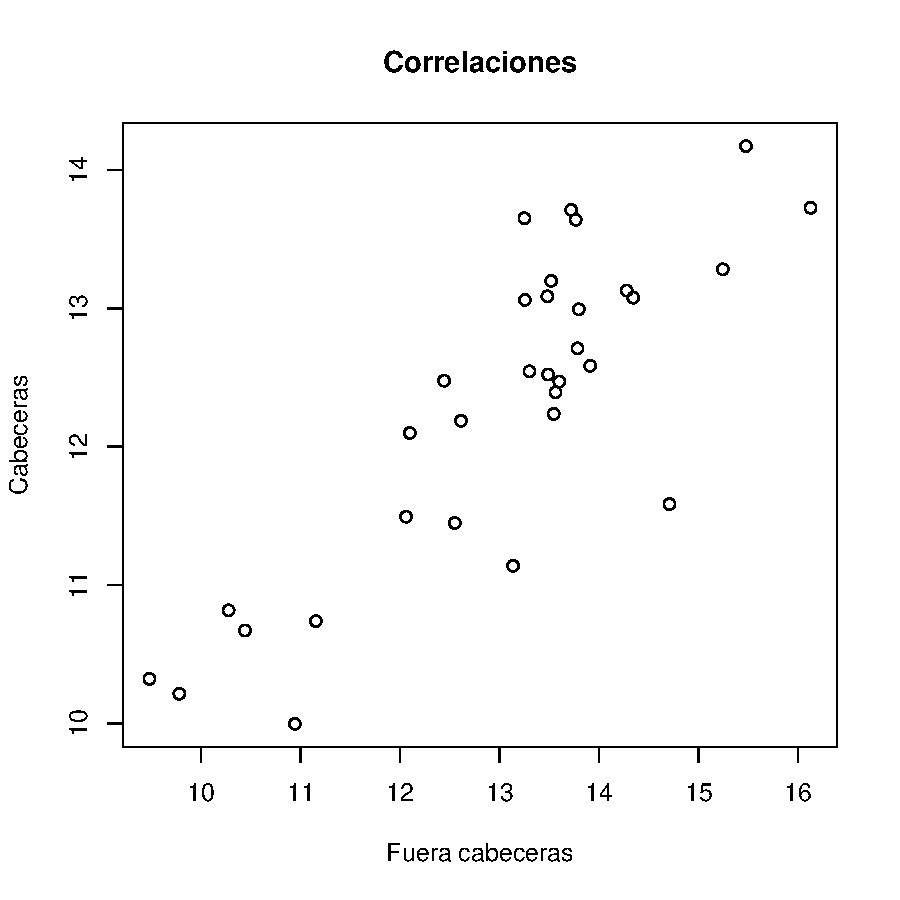
\includegraphics{Articulo1-corrPlotX}
\caption{correlación entre predictores}
\label{corrPlotX}
\end{figure}

\clearpage

\section{Modelos de Regresión}

Finalmente, vemos los modelos propuestos. Primero sin la libertad mundial como independiente, y luego con está. Los resultados se muestran en la Tabla \ref{regresiones} de la página \pageref{regresiones}.



% Table created by stargazer v.5.2.2 by Marek Hlavac, Harvard University. E-mail: hlavac at fas.harvard.edu
% Date and time: vie, jun 29, 2018 - 07:39:53 p.m.
\begin{table}[!htbp] \centering 
  \caption{Modelos de Regresión} 
  \label{regresiones} 
\begin{tabular}{@{\extracolsep{5pt}}lcc} 
\\[-1.8ex]\hline 
\hline \\[-1.8ex] 
 & \multicolumn{2}{c}{\textit{Dependent variable:}} \\ 
\cline{2-3} 
\\[-1.8ex] & \multicolumn{2}{c}{IDH} \\ 
\\[-1.8ex] & (1) & (2)\\ 
\hline \\[-1.8ex] 
 cabeLog & 0.013$^{***}$ & 0.031$^{***}$ \\ 
  & (0.004) & (0.007) \\ 
  & & \\ 
 restoLog &  & $-$0.030$^{***}$ \\ 
  &  & (0.010) \\ 
  & & \\ 
 Constant & 0.634$^{***}$ & 0.766$^{***}$ \\ 
  & (0.055) & (0.065) \\ 
  & & \\ 
\hline \\[-1.8ex] 
Observations & 32 & 32 \\ 
R$^{2}$ & 0.238 & 0.425 \\ 
Adjusted R$^{2}$ & 0.212 & 0.385 \\ 
Residual Std. Error & 0.037 (df = 30) & 0.033 (df = 29) \\ 
F Statistic & 9.347$^{***}$ (df = 1; 30) & 10.706$^{***}$ (df = 2; 29) \\ 
\hline 
\hline \\[-1.8ex] 
\textit{Note:}  & \multicolumn{2}{r}{$^{*}$p$<$0.1; $^{**}$p$<$0.05; $^{***}$p$<$0.01} \\ 
\end{tabular} 
\end{table} 
\clearpage

\section{Exploración Espacial}


Como acabamos de ver en la Tabla \ref{regresiones} en la página \pageref{regresiones}, si quisieras sintetizar la multidimensionalidad de nuestros indicadores, podríamos usar tres de las cuatro variables que tenemos (un par de las originales tiene demasiada correlación). 

Así, propongo que calculemos conglomerados de países usando toda la información de tres de los indicadores. Como nuestras variables son ordinales utilizaremos un proceso de conglomeración donde las distancia serán calculadas usando la medida {\bf gower} propuestas en \cite{macqueen_methods_nodate}, y para los enlazamientos usaremos la técnica de {\bf K-means}. Los tres conglomerados se muestran en la Figura \ref{clustmap}.



\begin{figure}[h]
\centering
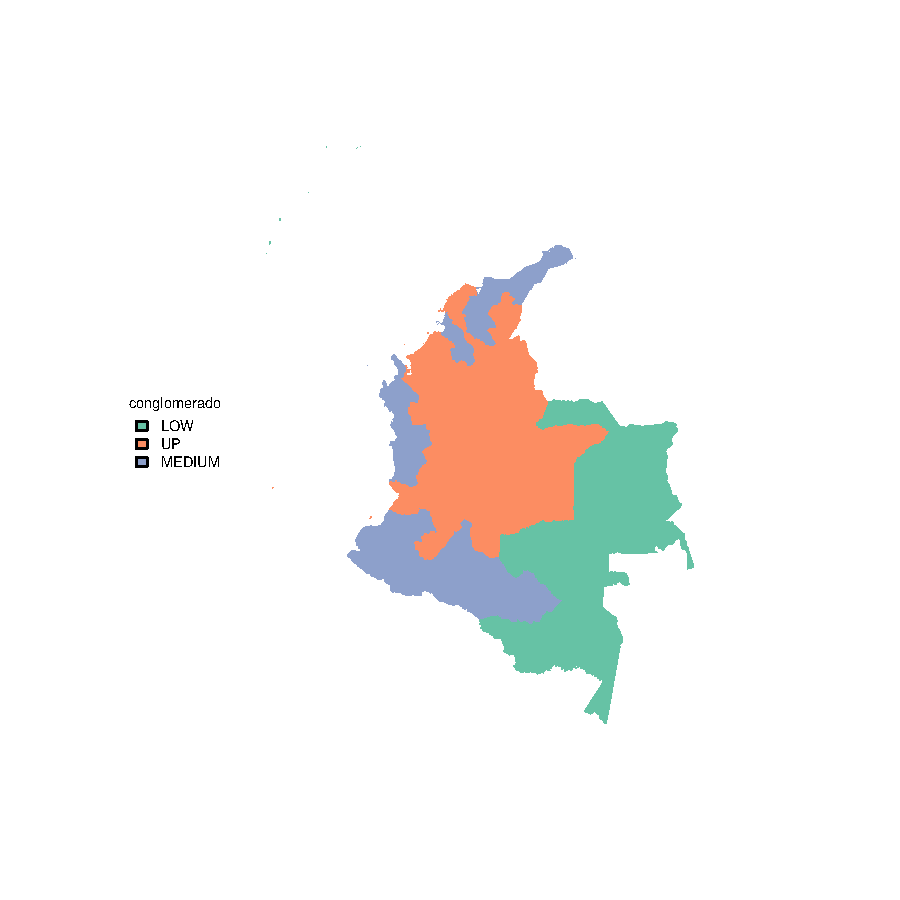
\includegraphics{Articulo1-plotMap1}
\caption{Departamentos conglomerados conglomerados segun sus indicadores sociopolíticos}\label{clustmap}
\end{figure}


\bibliographystyle{apalike}
\renewcommand{\refname}{Bibliografia}
\bibliography{Colombia1}

\end{document}
